\section{Lịch sử ngành lập trình di động}

  \hspace*{0.8cm}Ngành lập trình di động không xuất hiện một cách đột ngột, mà hình thành song song với sự phát triển của điện thoại di động qua từng thời kỳ. Từ những thiết bị to lớn, đắt đỏ và đơn chức năng, đến các smartphone hiện đại với khả năng xử lý mạnh mẽ và đa nhiệm, lập trình di động đã dần trở thành một lĩnh vực quan trọng trong ngành công nghệ thông tin. Việc hiểu rõ bối cảnh và các bước ngoặt trong lịch sử phát triển không chỉ giúp ta nhìn nhận đúng vai trò của lập trình di động, mà còn cho thấy những thách thức và cơ hội trong hành trình tạo ra các ứng dụng phục vụ hàng tỷ người dùng trên toàn cầu.

% 2.1
\subsection{Tổng quan về lịch sử ngành lập trình di động}
\renewcommand{\labelitemi}{--}  


  \hspace*{0.8cm}Lập trình di động là một lĩnh vực đã phát triển song hành với sự tiến hóa của thiết bị di động trong suốt nhiều thập kỷ. Từ những năm 1990, khi các thiết bị cầm tay đầu tiên như Nokia và BlackBerry bắt đầu phổ biến, nhu cầu về các phần mềm cơ bản như lịch, máy tính và trò chơi đơn giản đã thúc đẩy sự ra đời của các nền tảng lập trình di động ban đầu. Những ứng dụng này chủ yếu được viết bằng ngôn ngữ C hoặc Java ME, giới hạn bởi phần cứng yếu và màn hình nhỏ.

  \vspace{0.5em}

  \hspace*{0.8cm}Giai đoạn chuyển mình rõ rệt nhất của ngành bắt đầu từ năm 2007, khi Apple giới thiệu iPhone và hệ điều hành iOS. Sự xuất hiện của smartphone với màn hình cảm ứng, kết nối internet mạnh mẽ và kho ứng dụng trực tuyến đã tạo ra một bước ngoặt lớn. Ngay sau đó, Google ra mắt Android – một hệ điều hành mã nguồn mở, cho phép các nhà phát triển dễ dàng tạo ứng dụng và triển khai trên nhiều thiết bị khác nhau.

  \vspace{0.5em}

  \hspace*{0.8cm}Từ năm 2010 đến nay, lập trình di động đã trở thành một trong những lĩnh vực sôi động nhất của ngành công nghệ thông tin. Các công cụ phát triển như Android Studio, Xcode, cùng với các framework đa nền tảng như React Native, Flutter hay Xamarin, đã giúp rút ngắn thời gian phát triển và mở rộng khả năng tiếp cận người dùng. Đồng thời, những xu hướng mới như trí tuệ nhân tạo (AI), thực tế tăng cường (AR), và Internet vạn vật (IoT) cũng được tích hợp ngày càng sâu vào các ứng dụng di động.

  \vspace{0.5em}

  \hspace*{0.8cm}Có thể thấy, lịch sử ngành lập trình di động không chỉ phản ánh sự tiến bộ của công nghệ phần cứng và phần mềm, mà còn cho thấy vai trò ngày càng lớn của các ứng dụng trong đời sống hàng ngày. Hiểu rõ bối cảnh lịch sử này là cơ sở quan trọng để các nhà phát triển định hướng tương lai, lựa chọn công cụ phù hợp, và xây dựng các giải pháp sáng tạo đáp ứng nhu cầu người dùng hiện đại.


% 2.2
\subsection{Một số thiết kế của điện thoại di động qua từng thời kỳ}
\renewcommand{\labelitemi}{--}    
    
        \hspace*{0.8cm}Vào những năm 1980, những chiếc điện thoại di động đầu tiên ra đời với thiết kế to, nặng và thường phải mang theo như một chiếc túi xách. Các thiết bị này chủ yếu được sử dụng để nghe và gọi, không có màn hình hiển thị hoặc giao diện tương tác như hiện nay. Lúc này, khái niệm về lập trình di động vẫn chưa xuất hiện vì các thiết bị không hỗ trợ cài đặt thêm phần mềm.
    
        \vspace{0.5em}
    
      \hspace*{0.8cm}Đến thập niên 1990, cùng với sự phát triển của công nghệ vi mạch và màn hình LCD, điện thoại di động bắt đầu trở nên nhỏ gọn và phổ biến hơn. Các dòng máy như Nokia 3210 hay Motorola StarTAC không chỉ hỗ trợ gọi điện và nhắn tin, mà còn tích hợp một số ứng dụng đơn giản như đồng hồ báo thức, lịch và trò chơi Snake. Đây là thời kỳ lập trình di động bắt đầu hình thành, chủ yếu dưới dạng các phần mềm nhúng hoặc ứng dụng đơn giản viết bằng ngôn ngữ C hoặc Java ME.
  
      \vspace{0.5em}
  
    \hspace*{0.8cm}Giai đoạn tiếp theo bắt đầu từ năm 2007, khi Apple ra mắt iPhone – một thiết bị đánh dấu kỷ nguyên mới của điện thoại thông minh. Với màn hình cảm ứng đa điểm, hiệu năng mạnh mẽ và khả năng kết nối internet, iPhone đã thay đổi hoàn toàn cách người dùng tương tác với thiết bị di động \cite{iphone2007}. Sự ra đời của App Store vào năm 2008 đã mở ra một thị trường ứng dụng sôi động, thúc đẩy sự phát triển mạnh mẽ của lập trình di động. Gần như song song, Google cũng phát triển Android – hệ điều hành mã nguồn mở, cho phép các nhà sản xuất và lập trình viên tự do phát triển ứng dụng và tùy biến theo nhu cầu.


    %https://www.androidcentral.com/ac-readers-recall-their-very-first-cell-phones
    \begin{figure}[H]
      \centering
      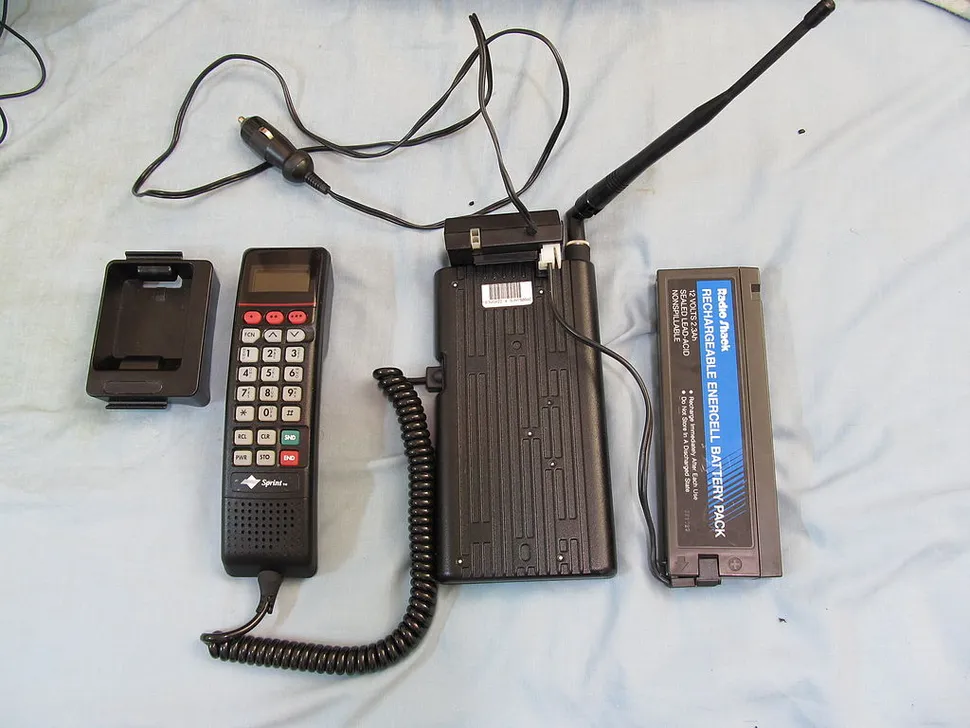
\includegraphics[width=0.75\textwidth]{images/thiet_ke_dtdd.png}
      \caption{Một số thiết kế điện thoại di động \cite{androidcentral2021}.}
      \label{fig:fig2}
    \end{figure}


  \hspace*{0.8cm}
  Từ năm 2010 đến nay, thiết bị di động đã đạt được những bước tiến vượt bậc về hiệu năng, độ phân giải màn hình, dung lượng pin và khả năng xử lý đa nhiệm. Các thiết bị ngày nay ngày càng có màn hình lớn và thời lượng sử dụng lâu dài, khiến chúng trở nên cồng kềnh. Đặc biệt, những thiết bị này, như iPad, có thể không cần áp vào tai mà vẫn cho phép người dùng thực hiện cuộc gọi. Bên cạnh đó, các công nghệ mới như trí tuệ nhân tạo (AI), thực tế ảo (VR), thực tế tăng cường (AR), và cảm biến sinh trắc học cũng được tích hợp sâu vào các thiết bị này, nâng cao khả năng sử dụng và ứng dụng. Bên cạnh đó, sự xuất hiện của các nền tảng phát triển đa nền tảng như React Native, Flutter và Xamarin đã tạo điều kiện thuận lợi cho các nhà phát triển viết ứng dụng một lần và triển khai trên cả iOS lẫn Android.

  \vspace{0.5em}

  \hspace*{0.8cm}Có thể thấy, thiết bị di động không ngừng được cải tiến cả về phần cứng lẫn phần mềm. Từ một công cụ liên lạc đơn giản, chúng đã trở thành trung tâm của mọi hoạt động số hóa trong đời sống hiện đại – từ học tập, làm việc, giải trí cho đến quản lý tài chính cá nhân. Quá trình phát triển qua các giai đoạn này không chỉ mở ra nhiều cơ hội cho lập trình viên, mà còn đặt ra những thách thức mới về hiệu suất, bảo mật và trải nghiệm người dùng.


% 2.3
\subsection{Motorola DynaTAC 8000X – Bước ngoặt đầu tiên của điện thoại di động}
\renewcommand{\labelitemi}{--}    

    \hspace*{0.8cm}Motorola DynaTAC 8000X, được giới thiệu vào năm 1983, là chiếc điện thoại di động thương mại đầu tiên trên thế giới. Thiết bị này đã đánh dấu một bước ngoặt quan trọng trong ngành viễn thông toàn cầu khi lần đầu tiên mang lại khả năng liên lạc di động thực sự cho người dùng cá nhân. Với hình dáng to lớn và trọng lượng nặng, DynaTAC vẫn nhanh chóng trở thành biểu tượng công nghệ của thời đại, đặt nền móng cho sự hình thành và phát triển sau này của các thiết bị di động thông minh cũng như ngành lập trình ứng dụng di động~\cite{motorola1983}.


% https://vi.m.wikipedia.org/wiki/T%E1%BA%ADp_tin:DynaTAC8000X.jpg
\begin{figure}[H]
  \centering
  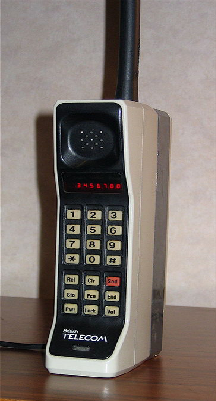
\includegraphics[width=0.25\textwidth]{images/DynaTAC8000X.png}
  \caption{Điện thoại Motorola DynaTAC 8000X \cite{wikiDynaTAC}.}
  \label{fig:fig4}
\end{figure}


  \hspace*{0.8cm}DynaTAC 8000X sở hữu thiết kế nổi bật theo phong cách công nghiệp, với kích thước khoảng 33 x 4.4 x 8.9 cm và trọng lượng lên đến 1.1 kg. Người dùng cần sử dụng cả hai tay để thao tác, khiến nó được gọi với biệt danh quen thuộc là “brick phone” – điện thoại cục gạch. Đây là minh chứng rõ rệt cho giai đoạn khởi đầu của công nghệ di động, khi tính cơ động vẫn còn là một khái niệm tương đối.

  \vspace{0.5em}

  \hspace*{0.8cm}Về mặt kinh tế, thiết bị này là một sản phẩm xa xỉ. Với mức giá lên tới \$3,995 vào năm 1983 (tương đương hơn \$10,000 hiện nay sau điều chỉnh lạm phát)~\cite{dynatacprice}, DynaTAC chỉ phù hợp với tầng lớp thượng lưu hoặc những người có nhu cầu đặc biệt. Không chỉ đắt đỏ về giá mua, người dùng còn phải trả thêm chi phí thuê bao hàng tháng và phí gọi tính theo phút – làm cho việc sử dụng thiết bị trở thành một khoản đầu tư lớn về tài chính.
  
  \vspace{0.5em}


  \hspace*{0.8cm}Về mặt kỹ thuật, DynaTAC không sở hữu màn hình màu, cảm ứng hay các chức năng nâng cao. Thiết bị chỉ phục vụ chức năng cơ bản là thực hiện và nhận cuộc gọi. Tuy nhiên, chính việc đưa công nghệ viễn thông ra khỏi không gian cố định – như điện thoại bàn – đã mở ra một thời kỳ hoàn toàn mới, trong đó việc giao tiếp trở nên linh hoạt hơn bao giờ hết. Đó là tiền đề quan trọng để những công nghệ di động sau này phát triển mạnh mẽ hơn.

  \vspace{0.5em}

  \hspace*{0.8cm}Tuy không hỗ trợ cài đặt phần mềm hay ứng dụng, DynaTAC vẫn có vai trò đặc biệt trong lịch sử lập trình di động. Sự xuất hiện của nó đã cho thấy tiềm năng thương mại rất lớn của các thiết bị cầm tay, từ đó thúc đẩy các nhà sản xuất phần cứng và kỹ sư viễn thông đầu tư vào nghiên cứu, phát triển hệ điều hành và nền tảng phần mềm cho thiết bị di động. Nhu cầu mở rộng chức năng thiết bị đã đặt nền móng cho việc phát triển các ứng dụng nhúng đầu tiên và các hệ điều hành cơ bản dành riêng cho di động.

  \vspace{0.5em}

  \hspace*{0.8cm}Nhìn một cách tổng thể, DynaTAC 8000X không chỉ là thiết bị điện thoại đầu tiên mà còn là biểu tượng khởi đầu của một ngành công nghiệp đầy tiềm năng. Mặc dù giới hạn về công nghệ và chức năng, sự thành công thương mại của nó đã truyền cảm hứng cho hàng loạt phát minh sau này – từ điện thoại thông minh cho tới hệ sinh thái lập trình ứng dụng di động đa dạng và phong phú như hiện nay.


% 2.4
\subsection{Từ “cục gạch” đến trải nghiệm người dùng hiện đại}
\renewcommand{\labelitemi}{--}    
    
        \hspace*{0.8cm}Sau khi điện thoại di động ra đời vào thập niên 1980, công nghệ đã không ngừng tiến hóa để biến những thiết bị vốn to lớn, nặng nề và đắt đỏ thành các sản phẩm nhỏ gọn, tiện lợi và phổ biến trong đời sống hàng ngày. Quá trình thu nhỏ phần cứng đi kèm với việc mở rộng khả năng xử lý và kết nối đã biến điện thoại di động từ một công cụ liên lạc thành một nền tảng công nghệ mạnh mẽ. Trong bối cảnh đó, trải nghiệm người dùng (User Experience – UX) dần trở thành một yếu tố trọng tâm, không chỉ trong thiết kế phần cứng mà còn trong quá trình phát triển phần mềm ứng dụng.
    
        \vspace{0.5em}
    
      \hspace*{0.8cm}Sự phát triển của UX trên thiết bị di động gắn liền với sự thay đổi trong hành vi và kỳ vọng của người dùng. Ban đầu, người dùng điện thoại di động chủ yếu mong muốn một thiết bị có thể thực hiện cuộc gọi ổn định và dễ sử dụng. Tuy nhiên, khi điện thoại trở nên phổ biến và chuyển mình thành điện thoại thông minh, người dùng bắt đầu kỳ vọng nhiều hơn: giao diện phải trực quan, tốc độ xử lý nhanh, thao tác mượt mà và trải nghiệm tổng thể phải liền mạch. Chính sự thay đổi về nhận thức và nhu cầu này đã thúc đẩy ngành lập trình di động phải chuyển hướng từ lập trình chức năng đơn thuần sang thiết kế lấy người dùng làm trung tâm.
    
      \vspace{0.5em}
    
      \hspace*{0.8cm}Việc điện thoại trở nên dễ tiếp cận hơn là một trong những yếu tố khiến UX trở thành một vấn đề cốt lõi. Nếu như những chiếc điện thoại đầu tiên có giá hàng nghìn đô la và chỉ phục vụ giới doanh nhân, thì ngày nay, người dùng ở mọi độ tuổi và tầng lớp xã hội đều có thể sở hữu ít nhất một thiết bị di động. Khi số lượng người dùng tăng lên, sự đa dạng về nhu cầu, trình độ công nghệ và thị hiếu sử dụng cũng trở nên phong phú hơn. Điều này tạo ra áp lực lớn đối với các nhà phát triển phần mềm, buộc họ phải tạo ra những sản phẩm vừa đơn giản, dễ dùng, vừa đầy đủ chức năng và mang lại cảm giác sử dụng thoải mái.
  
      \vspace{0.5em}
  
    \hspace*{0.8cm}Bên cạnh sự thay đổi của người dùng, sự tiến bộ nhanh chóng của phần cứng cũng là một yếu tố không thể bỏ qua. Các thiết bị hiện đại sở hữu màn hình độ phân giải cao, cảm ứng đa điểm, bộ xử lý mạnh, RAM lớn và pin dung lượng cao. Những tiến bộ này mở ra cơ hội cho các nhà phát triển phần mềm thiết kế giao diện ngày càng sinh động, đẹp mắt và tương tác tốt hơn. Nếu như trước đây ứng dụng di động chỉ có thể hiển thị văn bản đơn giản hoặc hình ảnh tĩnh, thì hiện nay, chúng có thể tích hợp video, hiệu ứng chuyển động, phản hồi xúc giác và thậm chí cả trí tuệ nhân tạo để cá nhân hóa trải nghiệm người dùng.
  
    \vspace{0.5em}
  
    \hspace*{0.8cm}Sự thay đổi lớn cũng diễn ra trong vai trò của các nhà sản xuất thiết bị di động. Trong giai đoạn đầu, các nhà sản xuất phần cứng thường là những người duy nhất phát triển phần mềm cho thiết bị của họ, từ giao diện người dùng cho đến các chức năng cơ bản. Tuy nhiên, mô hình này nhanh chóng bộc lộ hạn chế khi không thể đáp ứng kịp tốc độ thay đổi của thị trường và nhu cầu người dùng. Đồng thời, các nhà sản xuất cũng không sẵn sàng chia sẻ chi tiết về phần cứng của họ vì lý do bảo mật và cạnh tranh, khiến cho bên thứ ba rất khó tiếp cận và phát triển phần mềm.
  
    \vspace{0.5em}
  
    \hspace*{0.8cm}Chính sự bất cập đó đã làm nảy sinh một nhu cầu mới: cần có một lớp trung gian – hay chính xác hơn là một chuẩn kỹ thuật – giúp kết nối phần mềm với phần cứng một cách hiệu quả và an toàn. Các API (Application Programming Interface), SDK (Software Development Kit) và hệ điều hành di động như iOS hay Android đã ra đời nhằm mục đích đó. Chúng đóng vai trò là cầu nối giữa nhà sản xuất thiết bị và cộng đồng lập trình viên, giúp quá trình phát triển phần mềm trở nên dễ dàng hơn mà không cần phải hiểu sâu về kiến trúc phần cứng.
  
    \vspace{0.5em}
  
    \hspace*{0.8cm}Một trong những giải pháp mở đầu cho quá trình này là việc sử dụng trình duyệt web di động như một nền tảng để triển khai ứng dụng. Thay vì phát triển phần mềm cài đặt riêng biệt, các lập trình viên bắt đầu tối ưu hóa trang web để hoạt động tốt trên điện thoại. Từ đó, khái niệm “ứng dụng web di động” ra đời, đóng vai trò như bước chuyển tiếp giữa trình duyệt truyền thống và ứng dụng gốc (native app). Những trải nghiệm đầu tiên trên nền tảng web đã đặt nền móng cho việc hình thành tư duy thiết kế giao diện người dùng hiện đại.
  
    \vspace{0.5em}
  
    \hspace*{0.8cm}Nhìn chung, sự phát triển của UX trên thiết bị di động không chỉ phản ánh tiến bộ của công nghệ mà còn cho thấy mối liên kết chặt chẽ giữa phần cứng, phần mềm và hành vi người dùng. Việc đặt người dùng làm trung tâm không chỉ là xu hướng tạm thời mà đã trở thành triết lý phát triển cốt lõi trong ngành lập trình di động hiện đại. Từ “cục gạch” thô sơ ngày xưa đến những chiếc điện thoại tinh xảo hiện nay, trải nghiệm người dùng chính là yếu tố quyết định sự thành bại của một sản phẩm trong thời đại số.
  

% 2.5
\subsection{Chuẩn WAP – Khởi đầu cho trình duyệt web trên di động}
\renewcommand{\labelitemi}{--}    

  \hspace*{0.8cm}Trong những năm cuối thập niên 1990 và đầu những năm 2000, khi điện thoại di động bắt đầu được sử dụng rộng rãi trên toàn cầu, nhu cầu truy cập thông tin mọi lúc mọi nơi cũng trở nên cấp thiết. Tuy nhiên, hạ tầng mạng di động ở thời kỳ này lại chưa đủ phát triển: tốc độ kết nối rất chậm, băng thông hạn chế, và độ ổn định thấp. Vì vậy, việc sử dụng các trang web HTML tiêu chuẩn như trên máy tính là điều gần như không khả thi trên thiết bị di động lúc bấy giờ.
  
  \vspace{0.5em}
  
  \hspace*{0.8cm}Để giải quyết những hạn chế đó, chuẩn WAP – Wireless Application Protocol đã được ra đời như một giải pháp trung gian nhằm hiện thực hóa giấc mơ duyệt web trên thiết bị di động \cite{wap-intro}. WAP là một giao thức truyền thông được thiết kế đặc biệt cho môi trường mạng không dây với mục tiêu tạo điều kiện cho các thiết bị di động có thể truy cập, nhận và hiển thị dữ liệu từ các máy chủ web.
  

  % https://bkhost.vn/blog/wap-wireless-application-protocol/
\begin{figure}[H]
  \centering
  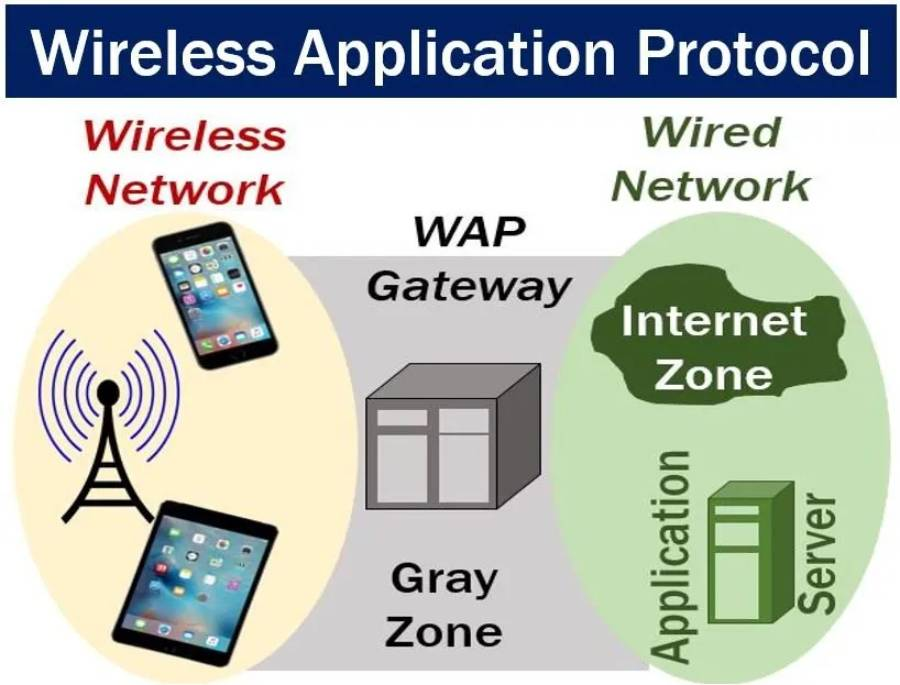
\includegraphics[width=0.7\textwidth]{images/Wireless-Application-Protocol-WAP-la-gi.jpg}
  \caption{Wireless Application Protocol (WAP) \cite{bkhostWAP}.}
  \label{fig:fig7}
\end{figure}
  
  
  \hspace*{0.8cm}Khác với giao thức HTTP vốn được xây dựng cho các máy tính kết nối mạng ổn định và tốc độ cao, WAP được ví như một “phiên bản rút gọn” của HTTP, tối ưu hóa cho việc vận hành trên các thiết bị có tài nguyên phần cứng hạn chế và kết nối mạng chậm như 2G hay GPRS \cite{wap-vs-http}. Nhờ vậy, dù rất đơn giản và sơ khai, WAP đã đóng vai trò như chiếc cầu nối giữa thế giới web truyền thống và thiết bị di động.
  
  \vspace{0.5em}
  
  \hspace*{0.8cm}Một trong những yếu tố then chốt làm nên hiệu quả của WAP chính là ngôn ngữ đánh dấu WML (Wireless Markup Language). Thay vì sử dụng HTML, vốn quá nặng và phức tạp với các thiết bị di động thời bấy giờ, WML được thiết kế nhẹ hơn nhiều, loại bỏ các yếu tố đồ họa và định dạng phức tạp \cite{wml-design}. Cú pháp của WML khá giống HTML nhưng bị giới hạn về số lượng thẻ và khả năng tương tác. Điều này cho phép hiển thị nội dung văn bản đơn giản như tiêu đề, đoạn văn, và các liên kết mà vẫn đảm bảo tốc độ tải nhanh và khả năng tương thích với phần cứng yếu.
  

  % https://learn.microsoft.com/en-us/archive/msdn-magazine/2001/june/net-mobile-web-sdk-build-and-test-wireless-web-applications-for-phones-and-pdas
\begin{figure}[H]
  \centering
  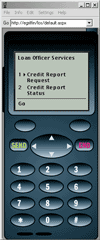
\includegraphics[width=0.2\textwidth]{images/cc301785.mobilefig02(en-us,msdn.10).png}
  \caption{Giao diện dịch vụ WAP Loan Officer trên điện thoại đời cũ \cite{msdnLoanOfficer}.}
  \label{fig:fig10}
\end{figure}
  
  
  \hspace*{0.8cm}Thêm vào đó, kiến trúc của WAP được xây dựng xoay quanh nguyên tắc tối ưu cho mạng yếu, nhằm giảm thiểu tối đa dữ liệu cần truyền và yêu cầu xử lý phức tạp. Nhờ đó, các thiết bị di động có thể tải và hiển thị nội dung một cách hiệu quả hơn, dù đang hoạt động trong điều kiện mạng không ổn định và băng thông hạn chế.
  
  \vspace{0.5em}
  
  \hspace*{0.8cm}Trong thời kỳ đầu, nhiều tổ chức và hãng thông tấn đã nhanh chóng nhận ra tiềm năng của WAP và bắt đầu phát triển các phiên bản website hỗ trợ giao thức này. CNN là một trong những đơn vị tiên phong, cung cấp nội dung tin tức thời sự cho người dùng di động thông qua nền tảng WAP. Tương tự, ESPN cũng phát triển phiên bản WAP nhằm cập nhật tỉ số thể thao và thông tin thi đấu cho khán giả thường xuyên di chuyển \cite{cnn-espn-wap}.
  
  \vspace{0.5em}
  
  \hspace*{0.8cm}Những ví dụ kể trên là minh chứng rõ ràng cho việc các nhà phát triển ứng dụng web đã bắt đầu chú trọng đến nền tảng di động, dù với rất nhiều giới hạn kỹ thuật so với web truyền thống trên máy tính. Tuy vậy, chính những nỗ lực này đã mở ra một hướng đi mới cho lĩnh vực phát triển ứng dụng – hướng đi mà sau này sẽ trở thành một trụ cột quan trọng trong ngành công nghệ.
  
  \vspace{0.5em}
  
  \hspace*{0.8cm}Xét về mặt lịch sử và ý nghĩa đối với lập trình di động, WAP có thể được xem là cột mốc đánh dấu sự khởi đầu của khái niệm "ứng dụng web di động". Nhờ vào chuẩn này, các lập trình viên thời kỳ đầu đã có môi trường và công cụ để bắt đầu phát triển nội dung dành riêng cho điện thoại di động, dù chỉ ở mức rất cơ bản.
  
  \vspace{0.5em}
  
  \hspace*{0.8cm}Không những thế, việc áp dụng WAP còn giúp định hình tư duy thiết kế ứng dụng tối giản, ưu tiên tốc độ và hiệu năng – một nguyên tắc vẫn còn giá trị trong phát triển ứng dụng di động hiện đại. Đồng thời, nó cũng mở ra kỷ nguyên mà điện thoại không chỉ là thiết bị nghe gọi, mà còn là cổng kết nối đến thế giới thông tin số – nơi người dùng có thể cập nhật tin tức, tra cứu thông tin, hay tương tác với nội dung web ở bất cứ đâu.
  

% 2.6
\subsection{Sự phát triển của thanh toán di động và bước ngoặt trong lập trình ứng dụng}
\renewcommand{\labelitemi}{--}


\hspace*{0.8cm}Khi điện thoại di động dần trở thành một phần thiết yếu trong đời sống hàng ngày, nhu cầu không chỉ dừng lại ở liên lạc mà còn mở rộng sang các tiện ích phục vụ tiêu dùng và giải trí. Trong quá trình phát triển đó, một yếu tố có vai trò đặc biệt quan trọng trong việc thúc đẩy sự bùng nổ của ứng dụng di động chính là khả năng thanh toán ngay trên thiết bị.

\vspace{0.5em}

\hspace*{0.8cm}Trong những ngày đầu, hình thức thanh toán thông qua SMS (Short Message Service) được xem là giải pháp khả thi nhất \cite{sms-payment}, bởi vì hầu hết các điện thoại di động đều hỗ trợ gửi và nhận tin nhắn. Với mô hình này, người dùng chỉ cần gửi tin nhắn đến một đầu số dịch vụ như 8xxx hoặc 6xxx để đổi lại các nội dung số như nhạc chuông, hình nền, hình động hay truyện cười. Khoản phí của tin nhắn này cao hơn nhiều so với tin nhắn thông thường và được tính trực tiếp vào tài khoản di động.

\vspace{0.5em}

\hspace*{0.8cm}Những tin nhắn dạng này được gọi là VAS – Value Added Services (dịch vụ giá trị gia tăng) \cite{vas-overview}, và chính chúng đã đặt nền móng cho mô hình kinh doanh nội dung số trên nền tảng di động. Đây cũng là lần đầu tiên mà lập trình viên có thể kiếm tiền thông qua các ứng dụng hoặc nội dung do họ xây dựng, dù vẫn còn ở dạng rất đơn giản.

\vspace{0.5em}

\hspace*{0.8cm}Khi điện thoại phát triển và người dùng ngày càng quen với việc tiêu dùng nội dung số, nhiều hình thức thanh toán khác cũng nhanh chóng ra đời để thay thế hoặc bổ sung cho SMS, tạo điều kiện mở rộng mô hình kinh doanh ứng dụng. Một trong số đó là thẻ cào điện thoại, cho phép người dùng nạp tiền vào tài khoản chính rồi sử dụng số dư này để mua vật phẩm hoặc dịch vụ trong game và ứng dụng \cite{prepaid-topup}.

\vspace{0.5em}

\hspace*{0.8cm}Tiếp theo là web charging, một hình thức thanh toán hiện đại hơn, cho phép người dùng mua nội dung trực tiếp trên website hoặc ứng dụng mà không cần can thiệp thủ công \cite{web-charging}. Khi người dùng chọn một dịch vụ trên trình duyệt hoặc trong app, hệ thống sẽ tự động trừ tiền vào tài khoản di động mà không yêu cầu xác nhận nhiều bước. Dù còn hạn chế và dễ phát sinh lỗi, web charging đã cho thấy tiềm năng to lớn của thương mại điện tử di động trong tương lai.

\vspace{0.5em}

\hspace*{0.8cm}Mặc dù các hình thức thanh toán kể trên còn đơn giản và chưa được bảo mật cao, nhưng chính chúng đã mở ra cánh cửa đầu tiên cho khái niệm “thanh toán di động”. Từ đó, lập trình viên không chỉ viết ứng dụng phục vụ giải trí mà còn có cơ hội tạo ra giá trị kinh tế thực sự, khuyến khích việc đầu tư bài bản vào thiết kế, trải nghiệm người dùng và chiến lược kiếm tiền.

\vspace{0.5em}

\hspace*{0.8cm}Song song với sự phát triển của các mô hình thanh toán, ngành lập trình di động cũng chứng kiến một bước chuyển mình mạnh mẽ. Khi người dùng tăng trưởng nhanh chóng và nhu cầu sử dụng di động vượt xa kỳ vọng, các công ty công nghệ lớn như Apple, Google, và sau này là Samsung, Huawei đã chính thức bước vào cuộc chơi với các hệ điều hành và nền tảng ứng dụng riêng biệt.

\vspace{0.5em}

\hspace*{0.8cm}Trước giai đoạn này, lập trình di động vẫn chủ yếu dựa vào nền tảng J2ME (Java 2 Micro Edition) – một môi trường phát triển cực kỳ rối rắm \cite{j2me-limitations}. Các lập trình viên phải đối mặt với hàng loạt thách thức: mỗi dòng điện thoại lại có độ phân giải khác nhau, hệ thống phím bấm không đồng nhất, dung lượng bộ nhớ thấp và phần cứng yếu. Công cụ hỗ trợ thì thiếu thốn, giao diện đơn điệu và không có khả năng tái sử dụng mã nguồn.

\vspace{0.5em}

\hspace*{0.8cm}Chỉ đến khi phần cứng của thiết bị di động có bước tiến vượt bậc – với màn hình cảm ứng lớn, bộ xử lý mạnh, bộ nhớ RAM dồi dào, cùng lúc đó là sự xuất hiện của iOS (Swift/Objective-C) và Android (Java/Kotlin) – lập trình viên mới thực sự có cơ hội khai phá sức mạnh của nền tảng di động một cách toàn diện. Giao diện đẹp hơn, tốc độ xử lý nhanh hơn và đặc biệt là hệ sinh thái phát triển (SDK, IDE, kho ứng dụng) đầy đủ và nhất quán, đã tạo ra một cuộc cách mạng trong phát triển ứng dụng.


% 2.7
\subsection{Thị trường di động trên toàn thế giới}
\renewcommand{\labelitemi}{--}    

  \hspace*{0.8cm}Trước năm 2010, khi khái niệm “smartphone” còn khá mới mẻ với phần lớn người dùng, thị trường điện thoại di động toàn cầu vẫn được dẫn dắt bởi những thương hiệu gắn liền với sự bền bỉ, phổ thông và dễ sử dụng. Nổi bật trong số đó, không ai khác chính là Nokia – “ông vua” không ngai của thời kỳ tiền smartphone.
  
  \vspace{0.5em}
  
  \hspace*{0.8cm}Nokia đã từng bước định hình trải nghiệm di động cho hàng triệu người dùng trên toàn thế giới, từ những chiếc điện thoại đen trắng cơ bản đến các dòng máy màu, hỗ trợ nhạc chuông đa âm, chơi game Java, cài đặt phần mềm và chụp ảnh. Những model như Nokia 1100, 6300, N70, N95 không chỉ phổ biến mà còn trở thành biểu tượng của một thời kỳ công nghệ giản đơn mà hiệu quả.
  
  \vspace{0.5em}
  
  \hspace*{0.8cm}Tại Việt Nam, Nokia chiếm trọn niềm tin của người dùng nhờ thiết kế chắc chắn, pin “trâu”, giá thành hợp lý và khả năng hoạt động bền bỉ trong nhiều năm. Sự phổ biến của thương hiệu này mạnh đến mức tên “Nokia” từng được dùng để gọi chung cho bất kỳ chiếc điện thoại nào, dù có thể đó là sản phẩm của hãng khác \cite{nokia-vietnam-popularity}.
  

  % https://vneconomy.vn/nokia-viet-nam-da-thanh-microsoft-mobile-viet-nam.htm
\begin{figure}[H]
  \centering
  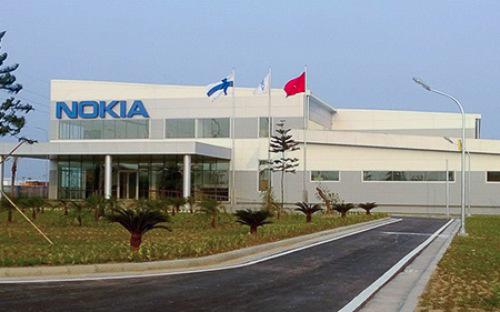
\includegraphics[width=0.75\textwidth]{images/nokia-4d687.jpg}
  \caption{Một nhà máy Nokia tại Việt Nam \cite{vneconomyNokia}.}
  \label{fig:fig8}
\end{figure}

  
  \hspace*{0.8cm}Song song với Nokia, các hãng như Blackberry, Sony Ericsson, Samsung, HTC cũng không ngừng nỗ lực chiếm lĩnh thị phần bằng cách phát triển các hệ điều hành riêng biệt hoặc hợp tác với bên thứ ba để tạo ra sự khác biệt. Một số nền tảng phổ biến lúc bấy giờ gồm:
  \begin{itemize}
  \item Symbian (Nokia)
  \item Blackberry OS (Blackberry)
  \item Windows Mobile, Windows CE (Microsoft)
  \item Palm OS, Linux Mobile, Bada OS (Samsung)
  \end{itemize}
  
  
  
  \hspace*{0.8cm}Tuy nhiên, một điểm yếu chung của tất cả các hệ điều hành kể trên chính là sự thiếu thống nhất và không thân thiện với lập trình viên. Mỗi hệ điều hành lại có giao diện riêng, API riêng, ngôn ngữ lập trình và tài liệu khác nhau – gây ra vô vàn khó khăn cho nhà phát triển:
  \begin{itemize}
  \item Trải nghiệm người dùng không đồng đều, giao diện không thống nhất.
  \item Bộ công cụ phát triển (SDK) còn sơ khai, thiếu tính năng và khó tiếp cận.
  \item Không có kho ứng dụng tập trung, dẫn đến việc phân phối phần mềm cực kỳ phức tạp \cite{pre-appstore-dev}.
  \item[]Điều này khiến phần lớn lập trình viên thời điểm đó vẫn còn thờ ơ hoặc làm việc theo kiểu "cho có", bởi chưa có hệ sinh thái đủ hấp dẫn để đầu tư nghiêm túc.
  \end{itemize}
  
  
  
  \hspace*{0.8cm}Mọi thứ chỉ thật sự thay đổi khi Apple chính thức ra mắt iPhone vào năm 2007. Thiết bị này không chỉ là một chiếc điện thoại thông minh đầu tiên theo đúng nghĩa hiện đại, mà còn là bước ngoặt vĩ đại của toàn ngành công nghiệp di động.
  
  \vspace{0.5em}
  
  \hspace*{0.8cm}Với màn hình cảm ứng đa điểm, thiết kế tinh tế không dùng bàn phím vật lý, hiệu năng mạnh mẽ và hệ điều hành ổn định, iPhone đã đặt ra một chuẩn mực mới cho smartphone. Tuy nhiên, cú hích lớn nhất chỉ đến vào năm 2008, khi App Store chính thức ra đời – nền tảng phân phối ứng dụng tập trung đầu tiên trong lịch sử di động.
  
  \vspace{0.5em}
  
  \hspace*{0.8cm}App Store không chỉ giúp người dùng dễ dàng tìm kiếm và cài đặt phần mềm, mà còn mở ra cơ hội kinh doanh ứng dụng chuyên nghiệp cho lập trình viên trên toàn thế giới. Với một bộ công cụ phát triển mạnh mẽ, tài liệu hướng dẫn đầy đủ và cộng đồng sôi nổi, iOS SDK đã biến lập trình di động từ một công việc khó khăn, mơ hồ thành một ngành công nghiệp sáng tạo thực thụ.
  
  \vspace{0.5em}
  
  \hspace*{0.8cm}Kể từ đây, lập trình ứng dụng di động bước sang một kỷ nguyên mới, nơi trải nghiệm người dùng, hiệu năng và hệ sinh thái phát triển đóng vai trò trung tâm. Cuộc đua giữa các nền tảng như iOS và Android cũng bắt đầu, tạo nên một trong những giai đoạn sôi động nhất trong lịch sử công nghệ di động.
  

% 2.8
\subsection{Thị trường và sự cạnh tranh trong ngành lập trình di động}
\renewcommand{\labelitemi}{--}    
    
        \hspace*{0.8cm}Khi thị trường thiết bị di động bắt đầu bùng nổ vào đầu thập niên 2010, ba ông lớn công nghệ là Microsoft, Apple và Google đã nhanh chóng bước vào một cuộc cạnh tranh gay gắt nhằm chiếm lĩnh thị phần trong cả phần cứng, hệ điều hành và hệ sinh thái ứng dụng. Mỗi công ty lựa chọn một chiến lược phát triển riêng biệt, qua đó không chỉ định hình diện mạo ngành công nghiệp di động mà còn tác động sâu rộng đến cách thức phát triển ứng dụng di động sau này.
    
        \vspace{0.5em}
    
      \hspace*{0.8cm}Trong ba ông lớn, Microsoft là cái tên bước vào cuộc chơi di động với nhiều tham vọng nhưng lại chậm chân. Sau khi nhận ra xu thế bùng nổ của smartphone, Microsoft đã tiến hành một thương vụ lớn vào năm 2013: mua lại bộ phận thiết bị và dịch vụ của Nokia với kỳ vọng tạo ra một hệ sinh thái Windows toàn diện, thống nhất từ máy tính, máy tính bảng đến điện thoại \cite{msft-nokia}. Triết lý phát triển "Windows Universal Platform" (UWP) – một ứng dụng chạy được trên mọi thiết bị – là nỗ lực nhằm tối ưu trải nghiệm lập trình viên và người dùng \cite{uwp-overview}. Tuy nhiên, Windows Phone lại xuất hiện quá muộn so với iOS và Android. Kho ứng dụng nghèo nàn, cộng đồng lập trình viên thiếu mặn mà, và mặc dù hệ điều hành này có trải nghiệm mượt mà, nhưng lại thiếu linh hoạt và không thể cá nhân hóa sâu \cite{windows-phone-fail}. Kết quả, Windows Phone dần bị người dùng quay lưng và cuối cùng bị khai tử, để lại một bài học sâu sắc về tầm quan trọng của thời điểm gia nhập thị trường và sự linh hoạt trong thích nghi với xu thế công nghệ.

      \vspace{0.5em}

      \hspace*{0.8cm}Một trong những nguyên nhân cốt lõi dẫn đến thất bại của Windows Phone nằm ở các quyết định chiến lược sai lầm trong thiết kế kiến trúc hệ điều hành. Dù sở hữu giao diện hiện đại và hoạt động ổn định, nền tảng này lại gây không ít khó khăn cho lập trình viên khi phát triển các ứng dụng có tính năng nâng cao. Một hạn chế nghiêm trọng là Windows Phone áp đặt mức giới hạn bộ nhớ RAM nghiêm ngặt: mọi ứng dụng không được sử dụng quá 300MB RAM, nếu vượt quá sẽ bị hệ điều hành tự động đóng. Trong khi đó, cả Android lẫn iOS đều cho phép ứng dụng khai thác tài nguyên một cách linh hoạt hơn, miễn là thiết bị vẫn còn đủ bộ nhớ. Sự cứng nhắc này khiến nhiều lập trình viên không thể triển khai những tính năng phức tạp hoặc tối ưu trải nghiệm người dùng như trên các nền tảng đối thủ, từ đó làm suy giảm sức hấp dẫn của hệ sinh thái Windows Phone đối với cộng đồng phát triển.
    
      \vspace{0.5em}
    
      \hspace*{0.8cm}Ngược lại với Microsoft, Apple là công ty dẫn đầu trong cả trải nghiệm người dùng lẫn xây dựng hệ sinh thái khép kín. Với triết lý thiết kế "từ trong ra ngoài" – nghĩa là kiểm soát cả phần cứng và phần mềm – Apple tạo ra sự đồng bộ, ổn định và an toàn cao cho các thiết bị của mình. iPhone nổi bật với thiết kế tinh tế, hiệu năng mượt mà; hệ điều hành iOS ít lỗi và có tính bảo mật cao; App Store được quản lý chặt chẽ, đảm bảo chất lượng ứng dụng. Đồng thời, Apple luôn chú trọng đến việc hỗ trợ lập trình viên thông qua các công cụ chuyên nghiệp như Xcode, ngôn ngữ Swift và các framework như UIKit hay SwiftUI \cite{apple-devtools}. Sự nhất quán này giúp Apple duy trì vị thế hàng đầu trong phân khúc smartphone cao cấp và sở hữu lượng người dùng trung thành cao bậc nhất thế giới.
    
      \vspace{0.5em}
    
      \hspace*{0.8cm}Về phía Google, chiến lược phát triển của họ xoay quanh triết lý mã nguồn mở, với Android là trung tâm của hệ sinh thái di động. Thay vì sản xuất phần cứng đại trà như Apple, Google phát triển Android như một nền tảng mở, cho phép các nhà sản xuất như Samsung, Xiaomi, Oppo hay Huawei tùy biến và tích hợp hệ điều hành này vào thiết bị của họ. Cách tiếp cận này giúp Android nhanh chóng chiếm lĩnh thị phần toàn cầu. Ban đầu, Android bị phê phán vì tính phân mảnh và kém ổn định, nhưng theo thời gian, Google đã liên tục cải tiến hệ điều hành qua từng phiên bản, siết chặt tiêu chuẩn chất lượng trên Google Play và giới thiệu dòng thiết bị Pixel nhằm kiểm soát tốt hơn trải nghiệm người dùng \cite{android-evolution}. Nhờ vào sức mạnh về dữ liệu, trí tuệ nhân tạo và mạng lưới dịch vụ (Gmail, Maps, YouTube...), Google vẫn giữ vững vị thế là trụ cột của ngành di động hiện đại.
    
      \vspace{0.5em}
    
      \hspace*{0.8cm}Sự cạnh tranh giữa Microsoft, Apple và Google – ba công ty với ba con đường phát triển khác nhau – không chỉ thúc đẩy đổi mới công nghệ mà còn tạo ra một hệ sinh thái lập trình di động phong phú, đa dạng và không ngừng phát triển. Chính sự đối đầu chiến lược này đã đặt nền móng cho những xu hướng lập trình đa nền tảng ngày nay.
    

% 2.9
\subsection{Hai hệ điều hành phổ biến nhất ngày nay: iOS và Android.}
\renewcommand{\labelitemi}{--}   

  \hspace*{0.8cm}Trong thị trường thiết bị di động hiện nay, iOS và Android là hai hệ điều hành chiếm lĩnh tuyệt đối, đồng thời là nền tảng chủ đạo cho việc phát triển ứng dụng di động trên toàn cầu. Mỗi hệ điều hành mang trong mình triết lý thiết kế, kiến trúc kỹ thuật và hệ sinh thái lập trình riêng, qua đó ảnh hưởng mạnh mẽ đến lựa chọn công cụ và quy trình làm việc của lập trình viên.


% https://www.ego-cms.com/post/5-major-differences-between-ios-and-android-app-development
\begin{figure}[H]
  \centering
  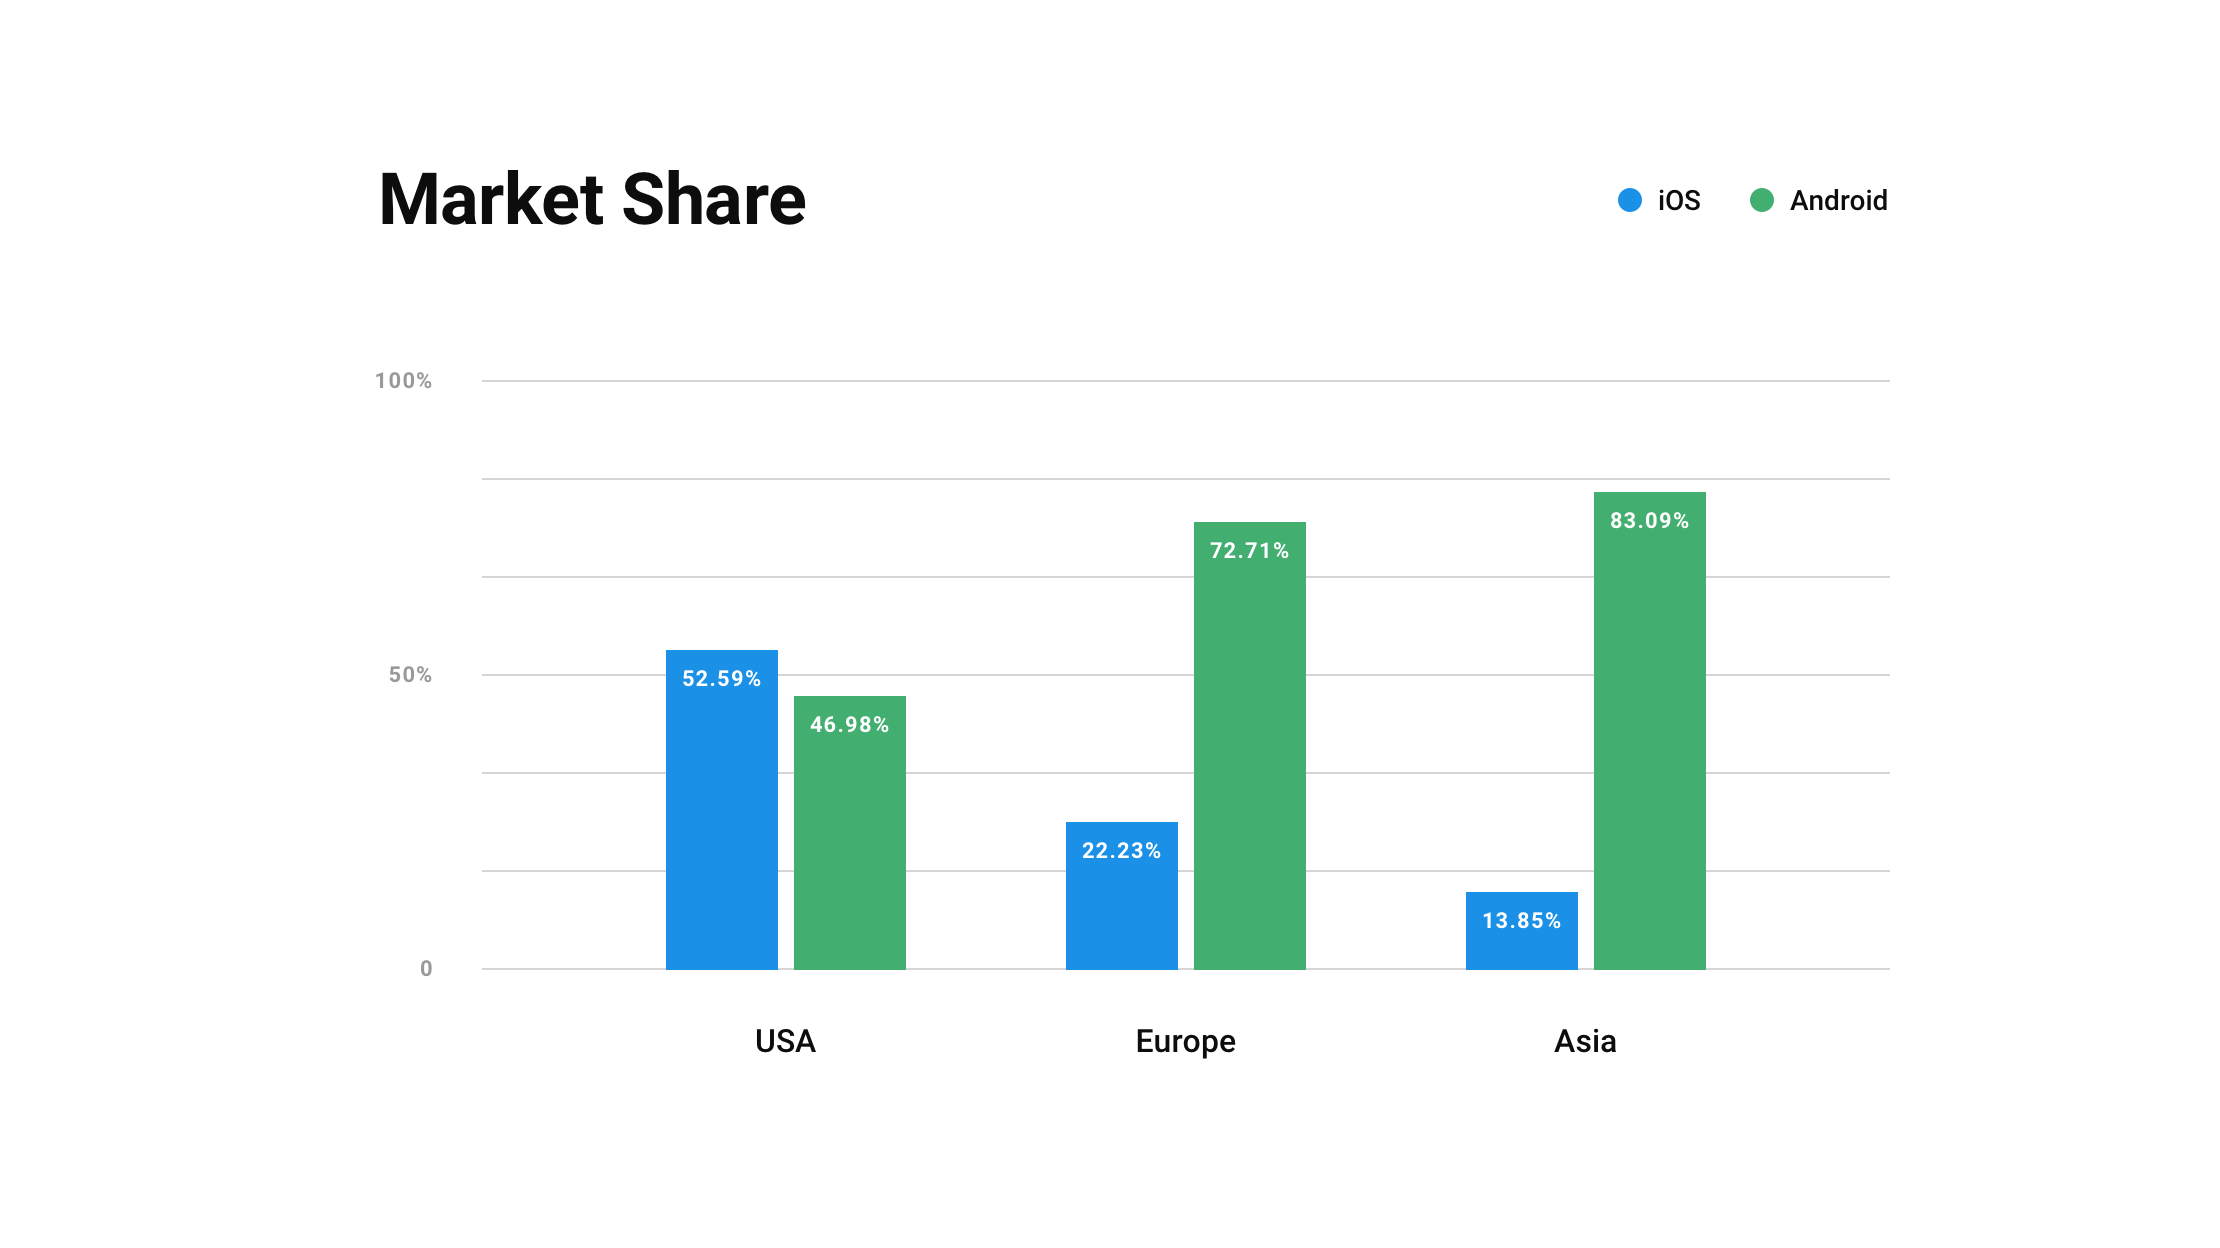
\includegraphics[width=0.8\textwidth]{images/Market Share.png}
  \caption{Chia sẻ thị trường giữa iOS và Android ở một số khu vực \cite{egoMarketShare}.}
  \label{fig:fig}
\end{figure}
    
        \hspace*{0.8cm}iOS là hệ điều hành được phát triển độc quyền bởi Apple, chủ yếu sử dụng trên các thiết bị như iPhone, iPad và iPod Touch. Đặc điểm nổi bật của iOS là sự ổn định, hiệu suất cao và mức độ bảo mật nghiêm ngặt, được đảm bảo bởi quy trình kiểm duyệt ứng dụng chặt chẽ trên App Store. Về mặt lập trình, trước đây iOS sử dụng Objective-C, nhưng kể từ năm 2014, ngôn ngữ Swift – hiện đại, dễ học và tối ưu hóa hiệu năng – đã dần thay thế và trở thành ngôn ngữ chính trong phát triển iOS \cite{swift}. Các công cụ hỗ trợ như Xcode đóng vai trò trung tâm trong quá trình phát triển, với khả năng mô phỏng, kiểm thử và tối ưu hóa ứng dụng. Ngoài ra, Apple cung cấp nhiều framework mạnh mẽ như UIKit và SwiftUI để xây dựng giao diện người dùng một cách linh hoạt \cite{swiftui}. Tuy nhiên, do hệ sinh thái đóng, lập trình iOS thường phụ thuộc hoàn toàn vào công cụ và quy định của Apple.
    
        \vspace{0.5em}
    
      \hspace*{0.8cm}Android, trái lại, là một hệ điều hành mã nguồn mở do Google phát triển, dựa trên nền tảng Linux. Sự cởi mở trong kiến trúc giúp Android được sử dụng trên hàng trăm thương hiệu thiết bị khác nhau như Samsung, Sony, Xiaomi, hay Oppo, từ đó tạo ra một thị trường đa dạng và cạnh tranh mạnh mẽ. Về ngôn ngữ lập trình, Android ban đầu sử dụng Java, nhưng từ năm 2017, Kotlin đã được Google công nhận là ngôn ngữ chính thức do khả năng viết mã ngắn gọn, an toàn và tương thích tốt với Java \cite{kotlin}. Android Studio là môi trường phát triển tích hợp chủ đạo, cung cấp nhiều công cụ hữu ích như trình giả lập thiết bị, Gradle để quản lý dự án, và Firebase để hỗ trợ backend. Nhờ tính chất mở, Android cho phép các nhà sản xuất tùy chỉnh sâu hệ điều hành, nhưng điều này cũng dẫn đến sự phân mảnh trong trải nghiệm người dùng và thách thức trong kiểm thử ứng dụng.
    
      \vspace{0.5em}
    
      \hspace*{0.8cm}Bên cạnh phát triển ứng dụng gốc (native) cho từng hệ điều hành, ngày càng nhiều lập trình viên lựa chọn các công cụ phát triển đa nền tảng để tiết kiệm thời gian và công sức. Các nền tảng như Flutter (Google), React Native (Meta), Xamarin (Microsoft) và Unity (phổ biến trong phát triển game) cho phép viết một lần, chạy trên nhiều hệ điều hành. Cụ thể, Flutter sử dụng ngôn ngữ Dart và nổi bật với hiệu suất mượt mà cùng giao diện đẹp \cite{flutter}; React Native dựa vào JavaScript, cho phép tái sử dụng logic ứng dụng từ web sang mobile \cite{reactnative}; Xamarin dùng ngôn ngữ C\# để tạo ứng dụng native cho cả iOS lẫn Android \cite{xamarin}; còn Unity, vốn mạnh trong phát triển trò chơi, cũng có thể tạo ra các ứng dụng tương tác cao \cite{unity}. Mặc dù các công cụ này mang lại lợi ích về năng suất, nhưng vẫn tồn tại một số hạn chế về hiệu năng và khả năng truy cập đến các API hệ thống sâu.
    
      \vspace{0.5em}
    
      \hspace*{0.8cm}Tóm lại, sự phát triển vượt bậc của iOS và Android, cùng với sự ra đời của các công cụ phát triển đa nền tảng, đã tạo nên một môi trường phong phú, năng động và đầy tiềm năng cho ngành lập trình di động. Việc hiểu rõ đặc điểm của từng hệ điều hành và lựa chọn công cụ phù hợp sẽ là yếu tố then chốt giúp lập trình viên tối ưu hóa hiệu quả và chất lượng sản phẩm.
    